\chapter{Subject Definition}
\label{chap:subject_def}

\epigraph{Scientific inquiry starts with observation. The more one can see, the more one can investigate.}{Martin Chalfie}

In a research internship, or indeed in any research activity, it's crucial to properly define the subject of the research, and to extract a precise problematic. That's why, during my first few weeks as an intern, and in this chapter of the report, I've endeavored to define this framework. To do so, I begin by recalling the subject as defined in my agreement: 

\noindent\hbox to \textwidth{\hrulefill}

\acrshort{nas} for \acrshort{llm} architectures is computationally prohibitive. In this work, we will investigate the use of efficient optimization algorithms (example: parallel fractal optimization) to reduce the latency of real-world commercial web-scale text prediction system. The goal of this work is to solve the \acrshort{nas} problem to find an architecture that when trained with data D and training algorithm A, produces a model that has similar accuracy but significantly reduced latency.
The tasks composting this work are summarized below:
\begin{itemize}
    \item Modeling and analysis of the \acrshort{nas} problem
    \item Solving of the problem using original and high-performance optimization algorithms
    \item Application to well known \acrshort{llm} such as GPT
    \item Application to logistics/transports problems
\end{itemize}
\noindent\hbox to \textwidth{\hrulefill}


From there, to understand fully the problems, it's important to define what are \acrshort{llm}, and what are the stakes of this fields. Then, we will take a look about the application to manufacturing or logistics contexts. Alike we will look at the \acrshort{autodnn} fields, with focus to \acrshort{nas} and \acrshort{hpo} problems, to locate the further work in a global litterature. With this, I can finally close this part with a precise search problematic, to drive my contribution.

%%--------------------SECTION : LLM---------------------%%
\section{Large Langage Models (LLM)}
\label{sec:llm}
\acrshort{llm} can be defined as \acrfull{dnn} using the \Gls{transformer} bloc for \acrfull{nlp} problems. For the next parts, it's important to understand the architecture of the \acrshort{llm}, after a brief reminder about \acrshort{dnn}. Due to computation limitation, a lot of research contribution are about the \Gls{fine_tuning}, defined in \ref{sec:fine_tune}. To pursue to the next section, I will finish with a light review and taxonomy of \acrshort{llm}. 

%%--------------------SUBSECTION : DNN---------------------%%
\subsection{\acrfull{dnn}}
\label{sec:dnn}
Like many fields, \acrshort{dnn} comes from biology-inspired design. In 1943,  Warren Mcculloch and Walter Pitts introduced the idea of logical calculus and computation, based on neural network, in article \cite{mcculloch_logical_1943}. The \acrfull{ann} aims to reproduce the cells of the brain to make a reasoning : the brain neuron is a node using a function to "activate" and the synapse is edge linking neurons to each others.  


The figure \ref{fig:artifical_neuron} show the structure of an artifical neuron, taking input $x_i$ and trainable weights $\omega_i$, including the biais $\omega_0$. The output of the neuron is expressed as : $\hat{y} = f(x,\omega) =  \sigma(\sum_{i=1}^n x_i \omega_i +\omega_0)$, with $\sigma(.)$ the activation function.

\begin{figure}[h]
    \centering
    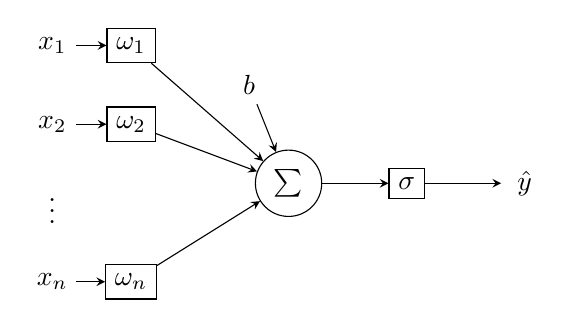
\begin{tikzpicture}[>=stealth, scale=1]

    % Define input nodes
    \node at (0, 1.5) {$x_1$};
    \node at (0, 0.5) {$x_2$};
    \node at (0, -0.5) {$\vdots$};
    \node at (0, -1.5) {$x_n$};

    % Define weight nodes
    \node[draw, rectangle] (w1) at (1, 1.5) {$\omega_1$};
    \node[draw, rectangle] (w2) at (1, 0.5) {$\omega_2$};
    \node[draw, rectangle] (wn) at (1, -1.5) {$\omega_n$};

    % Summation node
    \node[circle, draw] (sum) at (3, -0.25) {$\sum$};

    % Bias input
    \node at (2.5, 1.0) (b) {$b$};
    \draw[->] (b) -- (sum);

    % Sigma node
    \node[draw] (sigma) at (4.5, -0.25) {$\sigma$};

    % Output node
    \node at (6, -0.25) {$\hat{y}$};

    % Connect input to weights
    \draw[->] (0.3, 1.5) -- (w1);
    \draw[->] (0.3, 0.5) -- (w2);
    \draw[->] (0.3, -1.5) -- (wn);

    % Connect weights to summation node
    \draw[->] (w1) -- (sum);
    \draw[->] (w2) -- (sum);
    \draw[->] (wn) -- (sum);

    % Connect summation to sigma (activation function)
    \draw[->] (sum) -- (sigma);

    % Connect sigma to output
    \draw[->] (sigma) -- (5.7, -0.25);

\end{tikzpicture}
    \caption{Illustration of an artifical neuron}
    \label{fig:artifical_neuron}
\end{figure}


The activation function is the key of the \acrshort{ann}. The function need to make an output adapted to the use case (e.g. value between 0 and 1 for a probability), and to be differentiable to be able to use gradient-based optimization, the most efficient optimization method when possible. Approaches using \acrfull{ea} to update weights were studied and called \textit{meta-learning}\cite{hospedales_meta-learning_2022}, but were deprecated in favor of gradient-based methods. 

With the notation of figure \ref{fig:artifical_neuron}, and $\omega$ being the matrix of all parameters, the training of the \acrshort{ann} can be expressed as equation \ref{eq : ann_opt}. The loss $\mathcal L$ is the expression of the difference between the wanted output $y$ and the predicted output $\hat y$. Many formulas can be used the compute the loss, such as cross-entropy\cite{zhang_generalized_2018} or \acrfull{mse}.

\begin{equation}
    \omega \in \arg \min_{\omega \in \mathbb R^n} \mathcal L(\hat{y},y)
    \label{eq : ann_opt}
\end{equation}

The optimization of equation \ref{eq : ann_opt} is done using gradient descent, and especially \acrfull{sgd}. For each parameter, the gradient is expressed as \ref{eq : Gradient_descent}. Based on this, the parameter is updated with $\omega_{i} \gets \omega_i - \eta * \Delta_{\omega_i}$.

\begin{equation}
    \Delta_{\omega_i}=\Delta_{\omega_i}(x,y)=\frac{\partial \mathcal L(f(x,\omega),y)}{\partial \omega_i}
\label{eq : Gradient_descent}
\end{equation}

To accelerate the gradient descent, some optimization algorithm like \acrfull{adam} \cite{kingma_adam_2017} use the momentum of the function, replacing $\Delta \omega_i$ with $m_t = \beta m_{t-1}+(1-\beta)[\Delta \omega_i]$. In this formula, $m_t$ is the moment of the function $L$ at the instant $t$, and $\beta = [\beta_1, \beta_2]$ an hyperparameters of the method, with $\beta_i \in \{0,1\}$. In this internship, I will mostly use \acrshort{adam} or \acrshort{sgd}.

From simple \acrfull{mlp} to more complexe architecture (\acrfull{cnn}, \Glspl{transformer},\acrfull{vae}... ), from dozen to bilions of parameters, the \acrshort{dnn} are became over the years the \acrfull{sota} in many tasks : classification\cite{zhang_neural_2000}, computer vision\cite{rawat_deep_2017}, prediction \cite{khosravi_comprehensive_2011}, \acrshort{nlp}\cite{goldberg_primer_2016} etc.

%%--------------------SUBSECTION : Self Attention Mechanism---------------------%%
\subsection{Self Attention Mechanism}
\label{sec:self_att}


To understand how \acrshort{llm} works, it's crucial to understand the self attention mechanism. The key feature of \acrshort{llm} is the understanding of the context of a words to perform a prediction, or even a translation. Using \acrfull{mha}, the \textit{transformers} cells will define the importance of each words for the prediction of the next one. On the example of figure \ref{fig:self_att}, to predict the word "garden", the important words are "children" and "playing". The multiplicity of the attention head allow to understand different context with each one, like the color on the example. 

\begin{figure}[h]
    \centering
    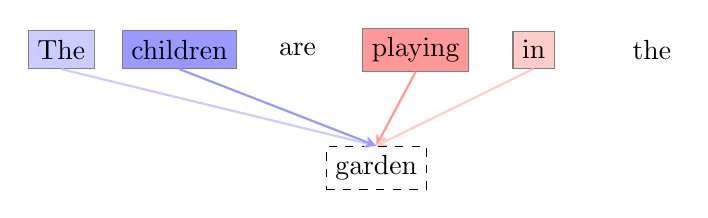
\begin{tikzpicture}[node distance=1.5cm]

% Define block styles
\tikzstyle{model} = [rectangle,rounded corners, minimum width=2cm, minimum height=1cm, text centered, draw=black, fill=blue!30]
\tikzstyle{arrow} = [thick,->,>=stealth]

% Define nodes
\node (the) [fill=blue!20,rectangle,draw=black!50] {The};
\node (children) [right of = the,fill=blue!40,rectangle,draw=black!50] {children};
\node (are) [right of = children] {are};
\node (playing) [right of = are,fill=red!40,rectangle,draw=black!50] {playing};
\node (in) [right of = playing,fill=red!20,rectangle,draw=black!50] {in};
\node (the2) [right of = in] {the};

\node (garden) [below of = are, xshift=1cm,rectangle,dashed,draw=black] {garden};

% Draw arrows
\draw [arrow,draw=blue!20] (the.south) -- (garden.north);
\draw [arrow,draw=blue!40] (children.south) -- (garden.north);
\draw [arrow,draw=red!40] (playing.south) -- (garden.north);
\draw [arrow,draw=red!20] (in.south) -- (garden.north);

% Add a rectangle around the last four nodes
\end{tikzpicture}
    \caption{Illustration of self attention}
    \label{fig:self_att}
\end{figure}


To perform this feat, Vaswani in article \cite{vaswani_attention_2017} present the scaled dot-product attention, used to build \acrshort{mha}. \Glspl{transformer} use a scaled dot-product attention, shown in figure \ref{fig:mha}, between a queries(Q)/Keys(K) pair, and a value (V) vector. With $d_k$ the dimension of the queries and keys,the attention function can be written as $Attention = \text{softmax} ( \frac{Q K^T}{\sqrt{d_k}})V$.

\begin{figure}[h]
    \centering
    \begin{tikzpicture}[node distance=0.8cm]

\tikzstyle{matmul} = [rectangle,rounded corners, minimum width=2cm , text centered, draw=black, fill=purple!30]
\tikzstyle{softmax} = [rectangle,rounded corners, minimum width=2cm , text centered, draw=black, fill=green!30]
\tikzstyle{mask} = [rectangle,rounded corners, minimum width=2cm , text centered, draw=black, fill=pink!30]
\tikzstyle{sca} = [rectangle, rounded corners, minimum width=2cm ,text centered, draw=black, fill=yellow!30]
\tikzstyle{action} = [rectangle, rounded corners, minimum width=2cm ,text centered, draw=black, fill=red!30]
\tikzstyle{arrow} = [thick,->,>=stealth]

\tikzstyle{linear} = [rectangle, rounded corners, minimum width=1cm ,text centered, draw=black, fill=blue!30]
\tikzstyle{dot-prod} = [rectangle, rounded corners, minimum width=2cm,minimum height = 1cm ,text centered, draw=black, fill=purple!50]
\tikzstyle{concat} = [rectangle, rounded corners, minimum width=2cm ,text centered, draw=black, fill=yellow!50]



% Define nodes
\node (matmul1) [matmul]{Matmul};
\node (softmax)[softmax, below of = matmul1, xshift = -0.8cm]{Softmax};
\node (mask) [mask, below of=softmax]{Mask (opt.)};
\node (scale) [sca, below of=mask]{Scale};
\node (matmul2) [matmul, below of=scale]{Matmul};
\node (q) [below of=matmul2, xshift=-0.5cm]{Q};
\node (k) [below of=matmul2, xshift=0.5cm]{K};
\node (v) [below of=matmul2, xshift=1.5cm]{V};


% Draw arrows
\draw [arrow] (matmul1.north) -- ([yshift=0.5cm]matmul1.north);
\draw [arrow] (softmax.north) -- ([xshift=-0.8cm]matmul1.south);
\draw [arrow] (mask.north) -- (softmax.south);
\draw [arrow] (scale.north) -- (mask.south);
\draw [arrow] (matmul2.north) -- (scale.south);
\draw [arrow] (q.north) -- ([xshift=-0.5cm]matmul2.south);
\draw [arrow] (k.north) -- ([xshift=0.5cm]matmul2.south);
\draw [arrow] (v.north) -- ([xshift=0.7cm]matmul1.south);


% MHA 
\node (linear1) [linear, right of = matmul1, xshift = 5cm] {Linear};
\node (concat) [concat, below of = linear1] {Concat};
\node (dot-prod) [dot-prod, below of = concat,yshift= -0.4cm] {Scaled Dot-product Attention};
\node (linear2) [linear, below of = dot-prod, xshift = -1.5cm, yshift = -0.4cm] {Linear};
\node (linear3) [linear, below of = dot-prod, yshift = -0.4cm] {Linear};
\node (linear4) [linear, below of = dot-prod, xshift = 1.5cm, yshift = -0.4cm] {Linear};
\node (q2) [below of=linear2]{Q};
\node (k2) [below of=linear3]{K};
\node (v2) [below of=linear4]{V};

% MHA arrow
\draw [arrow] (q2) -- (linear2);
\draw [arrow] (k2) -- (linear3);
\draw [arrow] (v2) -- (linear4);
\draw [arrow] (linear2.north) -- ([xshift=-1.5cm]dot-prod.south);
\draw [arrow] (linear3.north) -- (dot-prod.south);
\draw [arrow] (linear4.north) -- ([xshift=1.5cm]dot-prod.south);
\draw [arrow] (dot-prod) -- (concat);
\draw [arrow] (concat) -- (linear1);
\draw [arrow] (linear1.north) -- ([yshift=0.5cm]linear1.north);

% MHA * h
\node[draw, thick, dashed, rounded corners, fit=(dot-prod), inner sep=0.1cm, label=right:{$\times$ h}] {};
\node[draw, thick, dashed, rounded corners, fit=(linear2)(linear3)(linear4), inner sep=0.1cm, label=right:{$\times$ h}] {};


% Title
\node (dot_t) [above of = matmul1,yshift=0.5cm] {\textbf{Scaled Dot-Product Attention}};
\node (mha) [above of = linear1,yshift=0.5cm] {\textbf{Multi-Head Attention}};



\end{tikzpicture}
    \caption{\acrfull{mha} illustration }
    \label{fig:mha}
\end{figure}

The 3 linear cells are matrices multiplications between an input vector of size $d_i$ to a matrices $W^i \in \mathbb{R}{d_{model} . d_i}$, with $i \in {Q,K,V,O}$ ($O$ being the output vector). These matrices are the trainable weights of the Multi-Head Attention, and will be train along the rest of the network. The \acrshort{mha} output can be write as : 

\begin{equation}
\begin{split}
 Multihead (Q,K,V) = Concat (head_1,...,head_h)W^O\\
with \ head_i = Attention (Q W_i^Q,K W_i^K,V W_i^V)
\end{split}
\label{eq : MHA}  
\end{equation}

The softmax function is often used to extract probabilities, since it give values between 0 and 1, and that is take into account every values in order that the sum of softmax value is one. It can be written as : $\displaystyle
softmax(x_i) = \frac{e^{x_i}}{\sum_{j=1}^n e^{x_j}}$.

%%--------------------SUBSECTION : LLM architecture---------------------%%

\subsection{LLM Architecture}
\label{sec:llm_arch}
For many years, \acrshort{nlp} problems were approached by statistical and rules models, but they weren't able to capture the context of a whole sentence to generate a word. In 2016, Google published \textit{Google's Neural Machine Translation System} \cite{wu_googles_2016}, a \acrfull{lstm} neural network, trained on a big corpus of text datas, making it like the first \acrlong{llm}. This was an important break-through, and a proof-of-concept that neural networks can be the key of \acrshort{nlp} Problems.

To perform further, what \acrshort{nlp} needed was the ability to understand a context, to predict or understand a sentence. To do that, the \Gls{transformer} architecture was published in 2017 \cite{vaswani_attention_2017}, and was using the self attention mechanism presented in section \ref{sec:self_att}. 

\begin{figure}[h]
    \centering
    \begin{tikzpicture}[node distance=0.8cm]


\tikzstyle{norm} = [rectangle, rounded corners, minimum width=1cm ,text centered, draw=black, fill=red!30]
\tikzstyle{mha} = [rectangle,rounded corners, minimum width=2cm , text centered, draw=black, fill=orange!30]
\tikzstyle{feed} = [rectangle, rounded corners, minimum width=1cm ,text centered, draw=black, fill=blue!40]
\tikzstyle{embed} = [rectangle, rounded corners, minimum width=1cm ,text centered, draw=black, fill=pink!30]
\tikzstyle{encoding} = [rectangle, rounded corners, minimum width=1cm ,text centered, draw=black, fill=pink!40]
\tikzstyle{linear} = [rectangle, rounded corners, minimum width=1cm ,text centered, draw=black, fill=blue!20]
\tikzstyle{softmax} = [rectangle, rounded corners, minimum width=1cm ,text centered, draw=black, fill=green!20]


\tikzstyle{arrow} = [thick,->,>=stealth]
\tikzstyle{lightA} = [thick,dotted,->,>=stealth]

\tikzstyle{sum} = [circle, draw, minimum size=0.5cm, node distance=1cm, inner sep=0pt]

% Decoder node

\node (norm3)[norm,yshift = -0.5cm]{Add \& Norm};
\node (feed2)[feed,below of = norm3]{Feed-Forward};

\node (norm4)[norm,below of = feed2,yshift=-0.5cm]{Add \& Norm};
\node (mha2)[mha,below of = norm4]{MHA};

\node (norm5)[norm,below of = mha2,yshift=-0.5cm]{Add \& Norm};
\node (mha3)[mha,below of = norm5]{Masked MHA};

% Encoder node

\node (norm1)[norm,left of = norm4, xshift=-3cm]{Add \& Norm};
\node (feed1)[feed,below of = norm1]{Feed-Forward};

\node (norm2)[norm,below of = feed1,yshift=-0.5cm]{Add \& Norm};
\node (mha1)[mha,below of = norm2]{MHA};

% Arrow inside encoder
\node (enc_base)[below of = mha1]{};

\draw[lightA] (enc_base.center) -- (mha1);
\draw[lightA] (enc_base.center) -- ([xshift=-0.4cm, yshift = -0.4cm]mha1.south) -- ([xshift=-0.4cm]mha1.south);
\draw[lightA] ([yshift = -0.3cm]enc_base.center) -- (enc_base.center) -- ([xshift=0.4cm, yshift = -0.4cm]mha1.south) -- ([xshift=0.4cm]mha1.south);

\draw[lightA] ([yshift = -0.3cm]enc_base.center) -- ([yshift = -0.3cm,xshift = -1.3cm]enc_base.center) -- ([xshift = -1.3cm]norm2.center) -- (norm2.west);

\draw [lightA] (mha1) -- (norm2); 
\draw [lightA] (norm2) -- (feed1); 
\draw [lightA] (feed1) -- (norm1); 

\draw[lightA] ([yshift = 0.6cm]norm2.center) -- ([xshift = -1.3cm,yshift = 0.6cm]norm2.center) -- ([xshift = -1.3cm]norm1.center) -- (norm1.west);

\node(enc_fit)[draw, thick, dashed, rounded corners, fit=(norm1)(feed1)(norm2)(enc_base), inner sep=0.4cm, label=left:{N $\times$ }] {};

% Arrow inside decoder
\node (dec_base)[below of = mha3]{};

\draw[lightA] (dec_base.center) -- (mha3);
\draw[lightA] (dec_base.center) -- ([xshift=-0.4cm, yshift = -0.4cm]mha3.south) -- ([xshift=-0.4cm]mha3.south);
\draw[lightA] ([yshift = -0.3cm]dec_base.center) -- (dec_base.center) -- ([xshift=0.4cm, yshift = -0.4cm]mha3.south) -- ([xshift=0.4cm]mha3.south);

\draw[lightA] ([yshift = -0.3cm]dec_base.center) -- ([yshift = -0.3cm,xshift = 1.3cm]dec_base.center) -- ([xshift = 1.3cm]norm5.center) -- (norm5.east);

\draw [lightA] (mha3) -- (norm5); 

\draw [lightA] (norm5) --([yshift = 0.4cm]norm5.center) -- ([yshift=-0.4cm,xshift=0.4cm]mha2.south) -- ([xshift=0.4cm]mha2.south); 

\draw [lightA] (mha2) -- (norm4); 
\draw [lightA] (norm4) -- (feed2); 
\draw [lightA] (feed2) -- (norm3); 

\draw[lightA] ([yshift = 0.4cm]norm5.center) -- ([xshift = 1.3cm,yshift = 0.4cm]norm5.center) -- ([xshift = 1.3cm]norm4.center) -- (norm4.east);
\draw[lightA] ([yshift = 0.6cm]norm4.center) -- ([xshift = 1.3cm,yshift = 0.6cm]norm4.center) -- ([xshift = 1.3cm]norm3.center) -- (norm3.east);

\node(dec_fit)[draw, thick, dashed, rounded corners, fit=(norm3)(dec_base), inner sep=0.4cm, label=right:{$\times$ N}] {};

%arrow from encoder to decoder

\draw[arrow] (norm1.north) -- ([yshift=0.4cm]enc_fit.north)
    -- ([yshift=0.4cm, xshift = 2cm]enc_fit.north)
    -- ([yshift=-2.2cm, xshift = 2cm]enc_fit.north)
     -- ([yshift=-2.2cm, xshift = 3.8cm]enc_fit.north)
     -- (mha2.south);
\draw[arrow] ([yshift = -0.55cm, xshift = -0.4cm]mha2.south) -- ([xshift = -0.4cm]mha2.south);

% encoder input
\node (enc_plus) [sum, below of = enc_base,yshift=-0.1cm]{\Large $+$};
\node (in_embed) [embed, below of = enc_plus,align=center, yshift = -0.2cm]{Input \\ Embedding};
\node (encoding1) [encoding,left of = enc_plus, align = center, xshift = -1.5cm, yshift=-0.2cm]{Positional \\ Encoding};
\node (input) [below of = in_embed, yshift = -0.3cm]{Input};

% Decoder Input
\node (dec_plus) [sum, below of = dec_base,yshift=-0.1cm]{\Large $+$};
\node (out_embed) [embed, below of = dec_plus,align=center, yshift = -0.2cm]{Ouput \\ Embedding};
\node (encoding2) [encoding,right of = dec_plus, align = center, xshift = 1.5cm, yshift=-0.2cm]{Positional \\ Encoding};
\node (output) [below of = out_embed, yshift = -0.3cm, align = center]{Ouputs \\ (shifted right)};

%outputs
\node (linear) [linear, above of = norm3, yshift = 0.3cm]{Linear};
\node (softmax) [softmax, above of = linear]{Softmax};
\node (out) [above of = softmax,align = center, yshift=0.2cm]{Output \\ Probabilities};


% I/O arrow
\draw[arrow] (input) -- (in_embed);
\draw[arrow] (in_embed) -- (enc_plus);


\draw[arrow] (input.west) -- ([ yshift = -0.8cm]encoding1.south) -- (encoding1);
\draw[arrow] (output.east) -- ([ yshift = -0.8cm]encoding2.south) -- (encoding2);


\draw[arrow] (output) -- (out_embed);
\draw[arrow] (out_embed) -- (dec_plus);
\draw[arrow] (encoding1) -- (enc_plus);
\draw[arrow] (encoding2) -- (dec_plus);
\draw[arrow] (enc_plus) -- ([yshift = -0.3cm]enc_base.center);
\draw[arrow] (dec_plus) -- ([yshift = -0.3cm]dec_base.center);
\draw[arrow] (norm3.north) -- (linear);
\draw[arrow] (linear) -- (softmax);
\draw[arrow] (softmax) -- (out);
\draw[arrow] (out.north) -- ([yshift = 0.5cm]out.north);

% Encoder and Decoder Legend
\node [left of = enc_base,xshift= -2cm]{\textbf{Encoder}};
\node [right of = dec_base,xshift= 2cm]{\textbf{Decoder}};

\end{tikzpicture}
    \caption{\Glspl{transformer} topology (inspired by \cite{vaswani_attention_2017}}
    \label{fig:transformers}
\end{figure}

\Gls{transformer} architecture, as shown in figure \ref{fig:transformers}, is composed of 3 main components : embedding (including positional encoding), encoder and decoder. The embedding consist of representing the words in a vector space, using \textit{tokenizer} to encode the sentence.  Along with it, the positional encoding allow the model to keep the position of the token inside the model. A sinusoidal function is used for this, to stay on a relative position and not an absolute.

The encoder is a stack of \acrshort{mha} with feed-forward layers, with the addition of a residual connection and a normalization layer between the two. The output of the encoder is used as the input of second \acrshort{mha} of the decoder. Like the encoder, the decoder is a stack of \acrshort{mha} with feed-forward layers, but is composed of two \acrshort{mha}. The first one is masked, to learn only the part before the word to predict, and the second one is not masked to learn the whole sentence.

This topology is the base of \acrshort{llm}, with diversification on the number of layer, the number of head and the size of the embedding vector. It will be further discussed in section \ref{sec:llm_review}, but some model are using only part of the \gls{transformer} architecture, with the rise of \textit{encoder-only} and \textit{decoder-only} models.

\subsection{Fine-Tuning}
\label{sec:fine_tune}
As of today, the training of \acrshort{llm} is split is two phases : the pre-training and the \gls{fine_tuning}. The \textbf{Pre-training} is computationally very expensive, and only few companies can made one from scratch (OpenAI, Meta, Mistral ...). It also need an enormous corpus of data, often kept hidden from public. Model after pre-training are called \acrfull{gpt} model or foundation model. At this point, \acrshort{llm} are able to answer a prompt correctly, with a general amount of knowledge, but not to excel in a specific task.

\begin{table}[h!]
    \centering
    \begin{tabular}{|c|c|c|}
        \hline
        \textbf{Aspect} & \textbf{Pre-Training} & \textbf{Fine-Tuning} \\
        \hline
        Objective & General-purpose learning & Task/domain adaptation \\
        \hline
        Dataset & Large, diverse & Small, specific \\
        \hline
        Scale & High resource demand & Relatively efficient \\
        \hline
        Duration & Weeks to months & Hours to days \\
        \hline
    \end{tabular}
    \caption{Comparison Between Pre-Training and Fine-Tuning for LLMs}
    \label{tab:pretrain_vs_finetune}
\end{table}



After pre-training, the next stage, known as \textbf{\Gls{fine_tuning}}, is a lighter but equally crucial step that adapts the general knowledge in the model to perform well on specialized tasks. Figure \ref{fig:pretrain_finetune} and table \ref{tab:pretrain_vs_finetune} illustrate the scope of the fine-tuning process, in opposition to the pre-training process.

\begin{figure}[h]
    \centering
    \begin{tikzpicture}[node distance=1.8cm]

    % Define block styles
    \tikzstyle{model} = [rectangle,rounded corners, minimum width=2cm, minimum height=1cm, text centered, draw=black, fill=blue!30]
    \tikzstyle{data} = [rectangle, rounded corners, minimum width=2cm, minimum height=1cm,text centered, draw=black, fill=yellow!30]
    \tikzstyle{action} = [rectangle, rounded corners, minimum width=2cm, minimum height=1cm,text centered, draw=black, fill=red!30]
    \tikzstyle{arrow} = [thick,->,>=stealth]
    
    % Define nodes
    \node (model1) [data,align=center] {Model\\Random init};
    \node (data1) [model, below of=model1,align=center]{Pre-Training \\ Data Corpus} ;
    \node (pre-train)[action, right of=model1, xshift=1.5cm,yshift=-1cm]{Pre-Training};
    \node (model2) [model, right of=pre-train, xshift = 1.5cm, yshift=1cm ]{Pre-Trained Model};
    \node (data2) [data, below of= model2]{In-domain data};
    \node (fine-tuning)[action, right of = model2, xshift = 1.5cm,yshift=-1cm]{Fine Tuning};
    \node (model3) [model, right of=fine-tuning, xshift = 1.5cm,align=center ]{Fine-Tuned \\ model};
    
    
    % Draw arrows
    \draw [arrow] (data1) -- (pre-train);
    \draw [arrow] (model1) -- (pre-train);
    \draw [arrow] (pre-train) -- (model2);
    \draw [arrow] (model2) -- (fine-tuning);
    \draw [arrow] (data2) -- (fine-tuning);
    \draw [arrow] (fine-tuning) -- (model3);
    
    % Add a rectangle around the last four nodes
    \node[draw, thick, dashed, rounded corners, fit=(model2) (fine-tuning) (model3) (data2), inner sep=0.3cm, label=above:{Fine-Tuning Framework}] {};
\end{tikzpicture}
    \caption{Pre-Training and Fine-Tuning Framework}
    \label{fig:pretrain_finetune}
\end{figure}

Fine-tuning is often applied to refine the \acrshort{llm} responses by training it on domain-specific datasets or to improve its performance on specific tasks, such as medical diagnosis, legal document analysis, or customer service automation. Research, including studies like \cite{wei_finetuned_2022}, suggests that fine-tuning not only helps with task-specific adaptation but also enhances the model's generalization abilities. This process enables the model to transfer the foundational knowledge it learned in pre-training more effectively across a variety of prompts, making it more robust and adaptable. The table \ref{tab:pretrain_vs_finetune} summarize difference between \gls{fine_tuning} and \gls{pre-training}.



\Gls{instruction-tuning} is the process of \gls{fine_tuning} a pre-trained \acrshort{llm} using datasets composed of instruction-response pairs. The goal is to enhance the model's ability to follow natural language instructions effectively. This involves training the model to generate precise, contextually relevant, and human-aligned responses to a variety of prompts. \Gls{instruction-tuning} often uses datasets containing diverse tasks and instructions, enabling the model to generalize across different domains. 

%%%%%%%%%%%%%%%%%%%%%%%%%%%%%%%%%%%% PEFT %%%%%%%%%%%%%%%%%%%%%%%%%%%%%%%%%%%%%
\paragraph{\acrfull{peft}}

\acrshort{peft} methods are aiming to reduce the cost of \gls{fine_tuning}, and make it more accessible to a wider range of users. Article \cite{han_parameter-efficient_2024} make an exhaustive review of \acrshort{peft}, and is the base of this paragraph. The two main approaches to \acrshort{peft} are \textit{additive} and \textit{reparameterization} methods.

The \textit{additive} approach aims to add news weights or layers to the models, and train only theses weights. Popular method  use \textit{adapter} layers, adding layer between layers of the model, as shown in figure \ref{fig:adapter}. One con of this approach is the rise of the inference time implied by the addition of these layers to the model.


\begin{figure}[h]
    \centering
    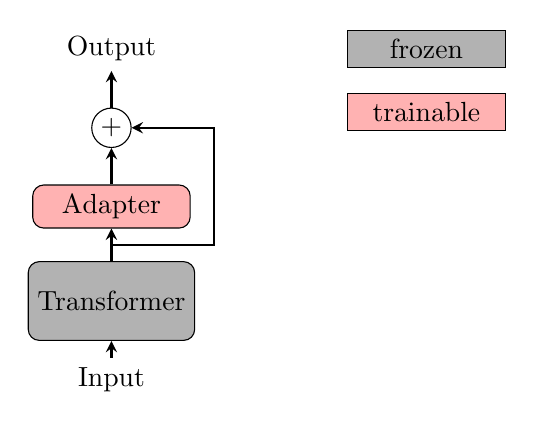
\begin{tikzpicture}[node distance=1cm]


    \tikzstyle{transformers} = [rectangle, minimum width=2cm ,text centered, draw=black, fill=black!30]
    \tikzstyle{adapter} = [rectangle, minimum width=2cm , text centered, draw=black, fill=red!30]
    \tikzstyle{arrow} = [thick,->,>=stealth]
    
    \tikzstyle{sum} = [circle, draw, minimum size=0.5cm, node distance=1cm, inner sep=0pt]
    
    % Define nodes
    \node (output)[]{Output};
    \node (plus)[sum, below of=output]{+};
    \node (adapter)[adapter,rounded corners, below of=plus]{Adapter};
    \node (transformer)[transformers,rounded corners, below of = adapter, minimum height=1cm, yshift=-0.2cm]{Transformer};
    \node (input)[below of = transformer]{Input};

    % vertical arrows
    \draw[arrow] (input) -- (transformer);
    \draw[arrow] (transformer) -- (adapter);
    \draw[arrow] (adapter) -- (plus);
    \draw[arrow] (plus) -- (output);

    % side arrow
    \draw[arrow] ([yshift=0.2cm]transformer.north) -- ([xshift= 1.3cm,yshift=0.2cm]transformer.north) -- ([xshift=1.3cm]plus.center) -- (plus.east);

    % legend block
    \node (frozen)[transformers, right of = output, xshift = 3cm]{frozen};
    \node (trainable)[adapter, below of = frozen, yshift = 0.2cm]{trainable};

    
\end{tikzpicture}
    \caption{illustration of adapter layer}
    \label{fig:adapter}
\end{figure}

The \textit{reparameterization} approach provide a proxy for model weights, to train this proxy and then merge it with the original model. The most popular method is \acrfull{lora}, based on article \cite{hu_lora_2021}. This method use the intrinsic rank of the weight matrix $W$, to factorize the matrix $W$ into 2 matrices $A$ and $B$ with $W = B.A$, with $W \in \mathbb{R}^{n*p}, A \in \mathbb{R}^{r*p} , B \in \mathbb{R}^{n*r}, r$ being the rank of the matrices factorization, as expressed in equation \ref{eq : lora}.

\begin{equation}
    \begin{split}
    W = W_0 + \Delta W = W_0 + B.A \\
    s.t. \quad W,W_0,\Delta W \in \mathbb{R}^{n*p},\\
    A \in \mathbb{R}^{r*p} \text{ and } B \in \mathbb{R}^{n*r}
    \end{split}
    \label{eq : lora}
\end{equation}

Figure \ref{fig:lora} show the illustration of the \gls{lora} layer, with $A$ and $B$ being the factorization of the weight matrix. The pros of this is the inference that aren't penalized since the model is composed of the same number of weights after the merging. Other pro it that multiple \gls{fine_tuning} can be effected and they can then be merged when it's needed from a same base, saving only the low-rank version of the weights. One con is that it add hyperparameters, but it will be tackled in nexts sections.

\begin{figure}[h]
    \centering
    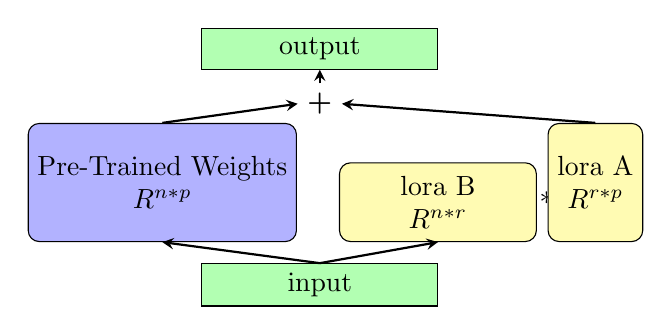
\begin{tikzpicture}[node distance=1.5cm]
    % Define block styles
    \tikzstyle{weights} = [rectangle,rounded corners, minimum width=2.5cm, minimum height=1.5cm, text centered, draw=black, fill=blue!30]
    \tikzstyle{lora_a} = [rectangle,rounded corners, minimum width=1cm, minimum height=1.5cm, text centered, draw=black, fill=yellow!30]
    \tikzstyle{lora_b} = [rectangle,rounded corners, minimum width=2.5cm, minimum height=1cm, text centered, draw=black, fill=yellow!30]
    \tikzstyle{vector} = [rectangle, minimum width=3cm, minimum height=0.5cm, text centered, draw=black, fill=green!30]
    \tikzstyle{arrow} = [thick,->,>=stealth]
    
    % Define nodes
    \node (weights) [weights, align=center]{Pre-Trained Weights \\ $\mathbb{R}^{n*p}$};
    \node (lora_B) [lora_b, right of=weights,xshift=2cm,yshift=-0.25cm, align=center]{lora B\\ $\mathbb{R}^{n*r}$};
    \node (mul) [right of = lora_B,xshift=-0.12cm]{*};
    \node (lora_A) [lora_a, right of=lora_B,xshift=0.5cm,yshift=0.25cm, align=center]{lora A\\$\mathbb{R}^{r*p}$};
    \node (input) [vector,below of = weights, xshift = 2cm,yshift=+0.2cm]{input};
    \node (plus) [above of = weights, xshift = 2cm,yshift=-0.5cm]{\textbf{+}};
    \node (output) [vector,above of = plus,yshift=-0.8cm]{output};
    
    
    
    
    % Draw arrows
    \draw [arrow] (input.north) -- (weights.south);
    \draw [arrow] (input.north) -- (lora_B.south);
    \draw [arrow] (weights.north) -- (plus.west);
    \draw [arrow] (lora_A.north) -- (plus.east);
    \draw [arrow] (plus) -- (output);
    
    
    \end{tikzpicture}
    \caption{illustration of lora layer}
    \label{fig:lora}
\end{figure}

In the litterature, somes articles before the emergence of \acrshort{llm} are using the terms "\gls{fine_tuning}" as the choice of \glspl{hyperparameter} like \acrfull{hpo}, but in this work, it will solely mean the second phase of \acrshort{llm} training.


\subsection{Review and taxonomy of LLMs}
\label{sec:llm_review}
Exhaustive review of LLMs can be found, like the article \cite{raiaan_review_2024}, with details on training, datasets, architectures... On this part, I will focus on key concept and details needed to achieve sufficient understanding for this report.

\paragraph{LLMs Taxonomy}
For this taxonomy, the criteria chosen is the downstream tasks, and the corresponding part of the Transformers Architecture used for this.\\
\textbf{Encoder-only} : LLMs using only the encoder side of the \textit{Transformers} are used to do text analysis or word classification (i.e. extract noun or verb of a sentence). The most famous one is BERT\cite{devlin_bert_2019} or its variations, an open source model by Google.\\
\textbf{Decoder-only} : these models are used for generative tasks, using prompts to lead it's generation. Generative Pre-Trained (GPT) models, with it's web service ChatGPT \cite{openai_gpt-4_2024} is a decoder-only model, and has strongly contribute to the renowned of the LLMs. We can also cite Llama \cite{grattafiori_llama_2024} family models, open-source foundation models.\\
\textbf{Encoder-Decoder} : model using standard Transformers are mainly used for translation, one of the first aim of NLP model, or summarize a text. BART\cite{lewis_bart_2020} or T5\cite{raffel_exploring_2020} models are fairly known model for this.

The relevance of this taxonomy come from the compatibility of different optimization method with these three types of models. Different types of models won't be used and train in the same way, and won't have the same hyperparameters. 

\paragraph{LLMs review}
In this part, I will briefly expose open issues concerning LLMs : \\
\textbf{Debiaising data corpus:} generative AI base it's representation on dataset, so it tend to reproduce the biaises of the corpus. For example, if we ask ChatGPT to generate 10 name of engineer, we have low probability of having parity.\\
\textbf{Interpretability :} using neural network in general, but especially LLMs, we can't explain why it works, or why a specific generation happens, so it has limited use.\\
\textbf{Efficiency and energy consumption :} the result-oriented search tend to only focus on accuracy, rather than energy consumption for a given result. This lead to an over and over-increase of the verticale networks size, and corresponding energy consumption to train and deploy it.\\
\textbf{Hallucinations\cite{bang_multitask_2023} :} when asking something to the model that does not have the answer, it tend to create a false answer from scratch, and be confident on it. It lower the confidence on the generation. 


%%--------------------SECTION : autoML---------------------%%
\section{Auto-DNN}
\label{sec:autodnn}
\acrfull{autodnn}, as defined in \cite{talbi_automated_2021}, refers to the automation of the design and optimization of deep neural network models. This concept is linked with \acrfull{automl}, but focus solely on \acrshort{dnn}. The contribution of \acrshort{autodnn} is multiples : 
\begin{itemize}
    \item Taking the human out of the loop, to find solutions outside of human expertise and way of thinking
    \item Ease the deployment of \acrshort{dnn} models, to lessen the needs of expertise
    \item Ensuring reliability and performance of the solution, with a data-driven approach
\end{itemize}

Two populars problem of this fields emerged in the last years : \textbf{\acrfull{nas}} and \textbf{\acrfull{hpo}}. In this part, I will briefly expose the general formulation of the \acrshort{autodnn} problem, and then focus on presenting \acrshort{nas} and \acrshort{hpo} specificities. 


%%-------------------- SUBSECTION : Problem Formulation---------------------%%
\subsection{Problem Formulation}
\label{sec : autodnn_pbm}
The general \acrshort{autodnn} optimization problem can be defined, like article \cite{talbi_automated_2021}, with a quadruplet $\alpha = (V,E,\lambda_V, \lambda_\alpha)$, where $V$ is a set of nodes denoting the neurons, $E$ is a set of edges (i.e. connections) between neurons, $\lambda_V$ the feature set of operations and $\lambda_\alpha$ the optimization features set of the \acrshort{dnn}. Given the space of all datasets $D$, the space of models $M$, and the search space of architectures $A$.

For reminder, namely $(x,y)$ the input-output pair, $f(x,\omega)=\hat{y}$ the predicted output and $\mathcal{L}(\hat{y},y)$ the loss function of the model. Subsequently to the optimization problem of section \ref{sec:dnn}, $\omega^*$ is the optimal parameters of the model.

Following the first optimization problem, a second is expressed as the \acrshort{autodnn} problem, with equation \ref{eq : autodnn_form}. In this equation, $f$ is the objective function, often the negative loss function or the accuracy. 

\begin{equation}
    a^* \in \text{arg max}_{a\in A}f(\Theta (a, d_{train}), d_{valid}= \text{arg max}_{a \in A} f(a).
    \label{eq : autodnn_form}
\end{equation}

The \acrshort{autodnn} problem is characterized, is the worst case, by theses properties : 
\begin{itemize}
    \item \textbf{\acrfull{mvop}} : Variables can be continuous (e.g. learning rate), discrete ordinal (e.g number of layers or neurons) or discrete categorical (e.g. type of activation function). The search space of the problem contains conditionnality, i.e. the size of a variables may depend on other variable (e.g. the number of neurons depend on the number of layers). These properties requires specific optimization methods, or conversion of variables.
    \item \textbf{Expensive black-box objective function :} this problem is a black-box function, i.e. the function cannot be analytically formulated, and so is derivative-free. The evaluation of a solution can take minutes to days, and even days, constraining the number of evaluations. These properties constrains optimization algorithms.  
\end{itemize}

\acrshort{autodnn} is an extremely broad field, and it's important to define precisely the specific problem we are treating. Following the notation of article \cite{elsken_neural_2019} about \acrshort{nas} problems, theses problems are structured according to three fields : \Gls{search_space}, \Gls{search_strat} and \Gls{perf_est}. The \textbf{\gls{search_space}} consists of all variables, and theirs properties (range, type ...). The \textbf{\gls{search_strat}} is about the optimization algorithms, defined more thoroughly in section \ref{sec : opt_algo}. The \textbf{\gls{perf_est}} is the definition of the loss function as expressed in equation \ref{eq : ann_opt}, and all linked attributes (e.g. datasets choice). This part can also includes approach like multi-fidelity, modifying the evaluation along iterations.



%%-------------------- SUBSECTION : NAS ---------------------%%
\subsection{\acrfull{nas}}
\label{sec : nas}

The \acrshort{nas} problem is a sub-problem of the \acrshort{autodnn} problem, where the search space is the topology \( G \) as defined in the preceding section. For an exhaustive survey of \acrshort{nas}, one can refer to the article by T. Elsken, *Neural Architecture Search: A Survey* \cite{elsken_neural_2019}. Figure \ref{fig:nas} presents the generic workflow of \acrshort{nas}. My contribution in this part focuses on \acrshort{nas} applied to \acrshort{llm}. Due to computational demands, the problem can be addressed using two approaches:

\begin{itemize}
    

    \item \textbf{Building from Scratch}:\\
    A classical approach to \acrshort{nas} involves building the architecture from scratch. However, the primary drawback of this method is the significant computational cost, making it accessible only to a limited number of organizations. A remarkable example of this is Google's development of the \textbf{AutoBERT-Zero} model \cite{gao_autobert-zero_2022}. This approach involves discovering an entirely new topology, including new transformer-based structures.\\
    To mitigate the computational cost, one can constrain the \gls{search_space}. For instance, the number of layers can be fixed, with modifications made to their internal components, or pre-built layers can be fixed, allowing experimentation with their arrangement.

    \item \textbf{Pruning}:\\
    Pruning involves reducing the size of a model by selecting parts of the topology while aiming to minimize performance degradation. A notable example of this is presented in \cite{klein_structural_2023}, which uses \textbf{weight sharing} methods, such as the approach proposed in \cite{pham_efficient_2018}.
\end{itemize}

\begin{figure}
    \centering
    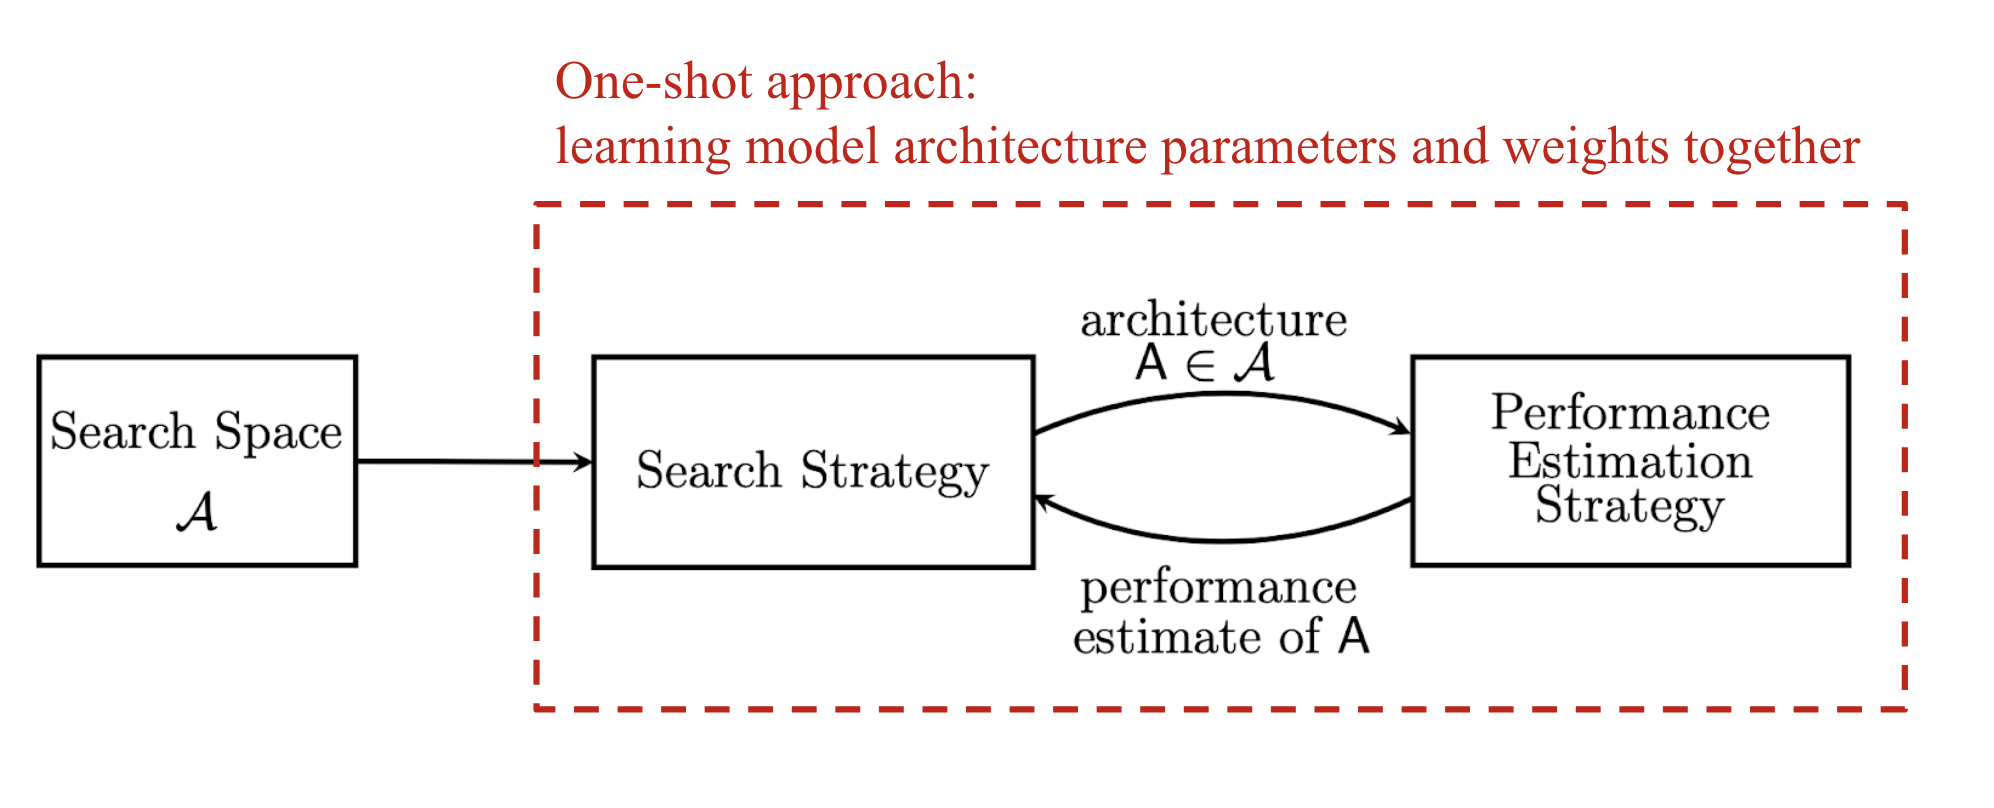
\includegraphics[width=0.6\linewidth]{assets/img/chap_2/NAS-high-level.png}
    \caption{Neural Architecture Search Workflow}
    \label{fig:nas}
\end{figure}

The methods to solve \acrshort{nas} for \acrshort{llm} are quite diverse. Some methods encode topology into a continuous space, broadening the range of possible optimization techniques. Further details will be addressed in Section \ref{sec : opt_algo}, but it is worth mentioning derivative-based methods like \cite{liu_darts_2019}, which apply such techniques to \acrshort{nas}.

%%-------------------- SUBSECTION : HPO ---------------------%%
\subsection{Hyper-parameter optimization}
\label{sec : hpo}
Like \acrshort{nas}, \acrshort{hpo} can be defined as a sub-field of \acrshort{automl}, even if \acrshort{hpo} by itself is tackled since the 1990s \cite{feurer_hyperparameter_2019}. In \acrfull{dnn}, \glspl{hyperparameter} can be defined as configuration settings that govern the structure of the networks and the process of training. As opposed to parameters (or weights), \glspl{hyperparameter} are not learning directly from the data during the training. They are typically set before training begins and remain fixed throughout the process.

Most of the time, \glspl{hyperparameter} are chosen by humans, w.r.t. their expertise. \acrshort{hpo} is the process of automating the choice of the best \glspl{hyperparameter} for a specific problem (a quadruplet $a$ as defined in \ref{sec : autodnn_pbm}). However, manually selecting \glspl{hyperparameter} is often inefficient and prone to suboptimal configurations, especially as models grow in complexity. Automated \acrshort{hpo} methods aim to address these challenges by systematically exploring the \gls{search_space} to identify configurations that maximize performance or minimize error for a given task.

The significance of \acrshort{hpo} grows with the increasing complexity of modern \acrshort{dnn} architectures. As models become larger and datasets more diverse, the choice of \glspl{hyperparameter} can significantly impact both model accuracy and computational efficiency. Moreover, \acrshort{hpo} plays a critical role in enabling the deployment of models in resource-constrained environments, where trade-offs between accuracy and efficiency must be carefully balanced. Future sections will detail methodologies and frameworks designed to tackle \acrshort{hpo} effectively in various contexts.



%%-------------------- SUBSECTION : Optimization Algorithms---------------------%%
\subsection{Optimization Algorithms taxonomy}
\label{sec : opt_algo}


Global optimization refers to the field of mathematical and computational methods designed to find the best solution to a problem within a defined domain, particularly when the objective function is complex, non-linear, or multi-modal. Traditional methods often struggled with problems involving multiple local optima or discontinuities. The search space $\mathcal X$ is generally a subspace of the real space $\mathbb{R}^n$, where $n$ is the dimensionality of the problem.

Optimization methods aim to efficiently navigate vast and complex search spaces, balancing the trade-off between \textit{exploration} (searching new regions) and \textit{exploitation} (refining known good solutions). In the context of hyperparameter optimization (HPO), global optimization plays a crucial role in systematically identifying configurations that maximize model performance while minimizing computational costs. The subsequent sections categorize and detail these optimization methods. 

\begin{equation}
    f(x) = (x_1^2 + x_2 - 11)^2 + (x_1 + x_2^2 - 7)^2
    \label{eq : himmelblau}
\end{equation}

In the next paragraphs, I will present a taxonomy of global optimization methods, w.r.t. their relevance in the \acrshort{hpo} problem. Equation \ref{eq : himmelblau} represent the \textit{himmelblau} function, a well-known non-convex function with multiple local optima. It will be used as an example in the following sections if relevant. 




\paragraph{Exploratory Methods} 
Basic approaches such as \acrfull{gs} (Grid Search) and \acrfull{rs} (Random Search) provide straightforward solutions for hyperparameter optimization (HPO). \acrshort{gs} systematically evaluates all possible combinations of hyperparameters within a predefined grid, making it simple to implement and interpret. However, this approach becomes computationally intractable in high-dimensional hyperparameter spaces due to the exponential increase in the number of configurations. On the other hand, \acrshort{rs} selects hyperparameters randomly from the search space, offering a more scalable alternative to \acrshort{gs} while maintaining simplicity. Despite its limitations, \acrshort{rs} is often used as a baseline or guideline to compare with more sophisticated optimization methods.


\begin{figure}[h]
    \centering
    \begin{subfigure}{.5\textwidth}
      \centering
      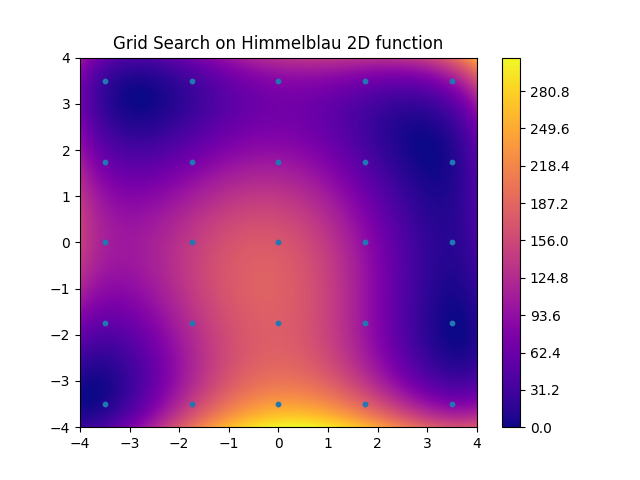
\includegraphics[width=\linewidth]{assets/img/chap_2/plots/grid_search.png}
      \caption{Grid Search}
      \label{fig:grid_search}
    \end{subfigure}%
    \begin{subfigure}{.5\textwidth}
      \centering
      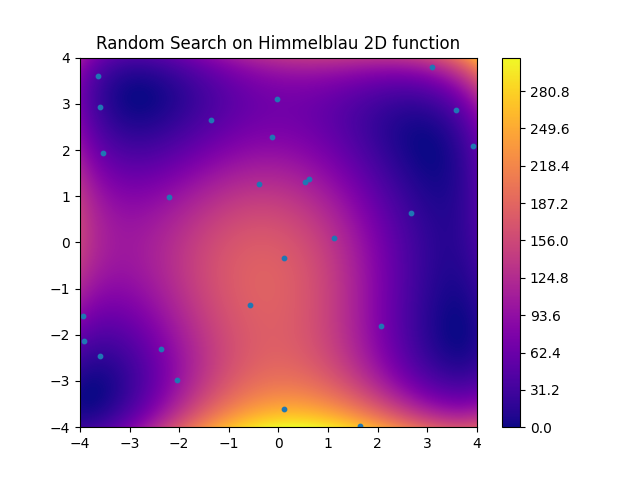
\includegraphics[width=\linewidth]{assets/img/chap_2/plots/random_search.png}
      \caption{Random Search}
      \label{fig:random_search}
    \end{subfigure}
    \caption{Exploratory Methods on Himmelblau 2D function}
    \label{fig:exploratory}
    \end{figure}

Figure \ref{fig:exploratory} show the results of the \acrshort{gs} and \acrshort{rs} on the \textit{himmelblau} function, with a given budget of 25 evaluations. Con of \acrshort{gs} is the curse of dimensionality, since with a grid of size $s$, the number of configurations to evaluate is $d^n$. \acrshort{rs} is less dependent on the dimensionality since the number of configurations to evaluate is only fixed by the budget. With search space including a lot of good solutions in the space, \acrshort{rs} can achieve efficient performance.

\paragraph{Metaheuristic Approaches}  

Metaheuristic methods, including \acrfull{sa} and \acrfull{ea}, are designed to search more efficiently within large hyperparameter spaces by mimicking natural or physical processes. \acrshort{sa} is inspired by the cooling process of metals, where the algorithm explores the search space by gradually reducing the probability of accepting worse solutions. This allows it to escape local optima and converge to a globally optimal solution over time. \acrshort{ea}, on the other hand, draw inspiration from biological evolution, employing operators such as mutation, crossover, and selection to iteratively improve a population of candidate solutions.

Metaheuristic can be classed on two main categories, population-based and solution-based. The first one like \acrshort{ga} are methods working on a population of candidate solutions, while the second one like \acrshort{sa} or \acrfull{ils} are methods working on a single solution. These approaches are particularly useful for complex, non-convex hyperparameter spaces where simpler methods like \acrshort{gs} or \acrshort{rs} might struggle.

\begin{figure}[h]
    \centering
    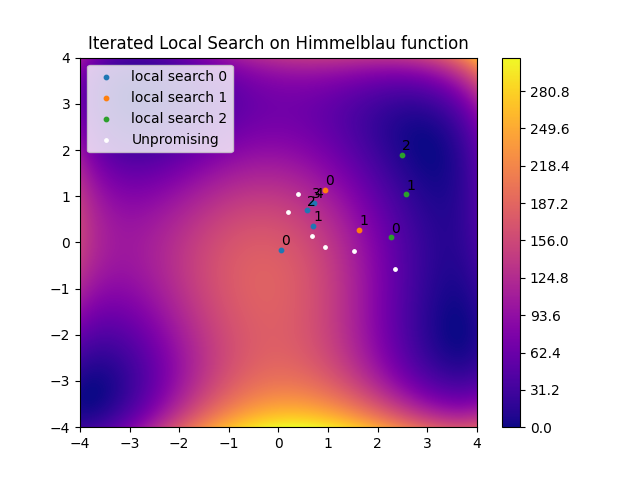
\includegraphics[width=0.5\linewidth]{assets/img/chap_2/plots/ils.png}
    \caption{Example of Iterated Local Search on himmelblau}
    \label{fig:ils}
\end{figure}

Even if theses methods are effective, they can be computationally expensive when dealing with expensive objective function evaluations, especially population-based methods. For a lot of methods like \acrshort{ils} in figure \ref{fig:ils}, unpromising evaluation are just discarded without really exploiting them. This characteristic makes them less suitable for high-dimensional hyperparameter spaces, and especially for \acrshort{hpo}.

\paragraph{\acrfull{pbo}}  

\acrfull{pbo} methods aim to divide the hyperparameter search space into smaller subspaces, focusing the search on the most promising regions. This division can be done either by penalizing less promising regions or by favorizing. Famous \acrshort{pbo} methods are \acrfull{fda}\cite{nakib_deterministic_2017}, DiRect \cite{jones_lipschitzian_1993} or even \acrfull{soo}\cite{munos_optimistic_2011}. One of the biggest advantages of \acrshort{pbo} methods is their intrinsicly parallelism abilities, enabling the scalibility of the optimization process when working with large hardware resources.

\begin{figure}[h]
    \centering
    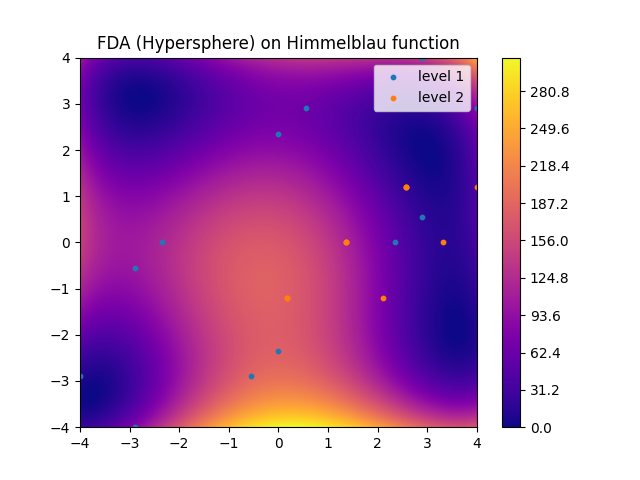
\includegraphics[width=0.5\linewidth]{assets/img/chap_2/plots/fda.png}
    \caption{Example of a Partition Based Optimization on 2D himmelblau}
    \label{fig:pbo}
\end{figure}

Figure \ref{fig:pbo} shows an example of \acrshort{pbo} algorithm, FDA using Hypersphere, on the \textit{himmelblau} function. Article \cite{firmin_comparative_2023} provides an exhaustive review and taxonomy of \acrshort{pbo} methods.


\paragraph{Surrogate-Model Based Optimization}  
Surrogate models, such as those employed in Bayesian Optimization (BO), offer a powerful framework for hyperparameter optimization. Instead of directly evaluating the objective function for every configuration, which can be computationally expensive, surrogate models approximate the objective function based on a limited number of evaluations. Gaussian Processes (GP), commonly used in BO, provide a probabilistic model of the objective function, capturing uncertainty and guiding the search toward the most promising regions of the hyperparameter space. Other surrogate models, such as tree-structured Parzen estimators (TPE), are also effective in optimizing complex, high-dimensional spaces. These methods are particularly advantageous when each evaluation of the objective function (e.g., training a machine learning model) is time-consuming or resource-intensive.
\begin{figure}[h]
    \centering
    %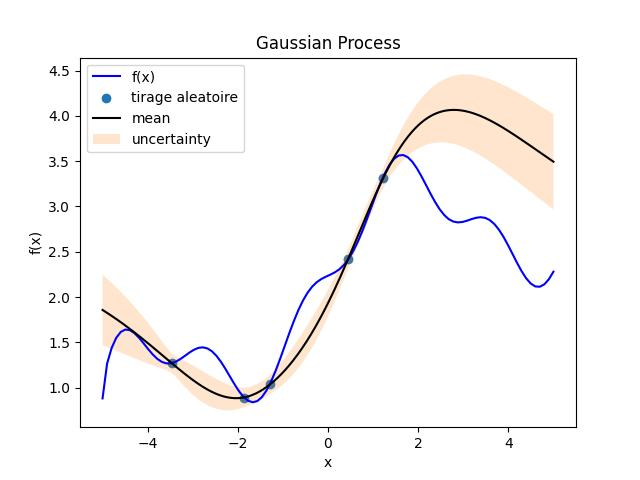
\includegraphics[width=0.5\linewidth]{assets/img/chap_2/plots/gaussian_process.jpg}
    \caption{Gaussian Process example}
    \label{fig:gp_eg}
\end{figure}




%%-------------------- SUBSECTION : Parallel and HPC ---------------------%%
\subsection{Parallel Optimization and High Performance Computing}

Parallel computation and high-performance computing (HPC) are fundamental to advancing artificial intelligence (AI). The complexity of optimization problems and resource demands of AI models necessitate parallel architectures, from multicore processors to distributed systems. Techniques like algorithmic and solution-level parallelism enable efficient exploration of massive search spaces, speeding up tasks such as evolutionary computation and deep learning optimization. Specialized hardware, such as GPUs and FPGAs, further accelerates matrix operations critical to AI workloads.

HPC platforms connect distributed clusters and grids, enabling scalable solutions to real-world challenges, including large-scale neural network training and hyperparameter optimization. NumPEx, through its Exa-MA (Methods and Algorithms for Exascale) subprogram, addresses computational challenges of exascale systems by developing scalable algorithms and architectures. Your work aligns with Exa-MA’s goals of advancing energy-efficient methods and leveraging HPC for predictive modeling, strengthening the synergy between AI innovation and exascale computing.


%%-------------------- SECTION : LLM to manufacturing ---------------------%%
\section{LLMs application to manufacturing context}
\label{sec:llm_manufacturing}
To link this internship to my engineering curriculum, I will explore the application for LLMs to manufacturing. The application can be split in three : quality control, Supply-chain management, predictive maintenance. Among these application, the two key-point of LLMs are the extensive reasoning, that can be used for prediction or analysis, and the performance in NLP problems, proving itself to be able to simply interact with any operators.

%%-------------------- SUBSECTION : LLM Quality Control ---------------------%%
\subsection{LLMs-based quality control}
\label{sec:llm_quality}
Quality control can be defined as \say{procedure or set of procedures intended to ensure that a manufactured product or performed service adheres to a defined set of quality criteria or meets the requirements of the client or customer} \cite{whatis_QC}. In this field, the last decades was really interesting from a data management point of view, since it's was the emergence of a lot of data collection : product measurement along manufacturing executive system (MES), customer feedbacks... Since a lot of unstructured data is collected, deep learning can be a way to use all of these to manage quality control. We can extract few specific ways : 

\begin{itemize}
    \item Automated Inspection : LLM are more and more multimodals, and it's possible to achieve computer vision along the reasoning capacities. It's now possible to go further and use camera to control every products on a conveyor. 
    \item Customer Feedback : LLM can be used to summarize and prioritize feedback, to be able to use precise insight on the manufacturing process.
\end{itemize}

%%-------------------- SUBSECTION : LLM Supply ---------------------%%
\subsection{LLMs-based supply chain management}
\label{sec:llm_scm}
Since decades, \textbf{demand forecast} is a hot field of supply chain management, with many methods considering means and data collection of the company. LLMs, and in specific time-LLM \cite{timeLLM_2024}, achieve a new step in automated reasoning, and to the corpus of data taken into account. From the first method using only historical sales, it's now possible to use a wider historical data, like climate, economical situation ... LLM can also be used for \textbf{supplier evaluation}. When considering a relationship with a supplier, many information can be used to characterise it : prices, delay, defaults, reactivity ... And LLM can summarize all of this to provide insight for the choice of a supplier on a specific project.   


%%-------------------- SUBSECTION : LLM Predictive Maintenace-----------------%%
\subsection{LLMs-based predictive maintenance}
\label{sec:llm_pred_maint}
By combining keys aspect of automated inspection and demand forecast, LLM could be a great asset in \textbf{maintenance scheduling}. One key point of these model is that they could use every possible inputs : machine logs, humain report, captures... With this, they could reach the best of humain (multi-modality) and machine (long, tedious tasks) to achieve state-of-the-art performance on these subject. More over, LLMs can be used for \textbf{root cause analysis}, to find the root of anomaly or failure and reduce the down time of the manufacture. 

%%-------------------- SECTION : Search Problematic ---------------------%%
\section{Search problematic}
My first two weeks were focus on understanding the context of the internship, mainly by reading articles, and working on extracting only one search problematic. To do this, my main concerns were : 
\begin{itemize}
    \item Feasibility : 24 weeks can be short for a too long research plan, all the more with long experiments. I need to be able to understand and assess the problem, try and implement methods.
    \item Costs : can't buy or build supercomputer just for this, and the cost of long computing of the resource can't be ignored 
    \item Research team expertise : the team is firstly optimization oriented, so problematic only oriented to LLMs won't be the priority
\end{itemize}

After a first week, the possible fields was narrowed to two tracks. The first one is based on article \cite{klein_structural_2023}, and involve the pruning of a large pre-trained model, in order to reduce latency without losing to much accuracy. The other one \cite{tribes_hyperparameter_2024} is Hyper-parameter Optimization (HPO) applied to Instruction tuning.  

Eventually, after reflection and discussion with my tutor, we choose to address the \acrshort{hpo} of \acrshort{llm} \gls{fine_tuning}. This choice was made to reduce the uncertainty on an already very exploratory fields, since \acrshort{hpo} was already tackled on different type of \acrshort{nn}. 

The objective of my internship is then to work on \acrshort{hpo} methods like apply to \acrshort{llm} \gls{fine_tuning}. This work includes : 
\begin{itemize}
    \item \textbf{Reproduce the objective function :} on a given library, implement the black box function of training and evaluate a \acrshort{llm}.
    \item \textbf{Definition of the search space : }balancing between curse of dimensionnality and research ambition, find pertinent \glspl{hyperparameter} to work with, and define theirs properties.
    \item \textbf{Selection and Implementation of Optimization algorithm :} considering litterature and available frameworks, choose relevant algorithms and implement it to the problem
    \item \textbf{Make experiments :} following a rigorous protocol, make experiments to determine the effects of the optimization, and analysis it
    \item \textbf{Formalize the contribution :} With this report and a scientific article, explicit the contribution, and formalize for furthers works
\end{itemize}

